\newpage
\section{Simulating circuits \label{sec:simulating_circuits}}
Oleg went  through how one  would simulate a  circuit, such as  the one
below (in fact this is the setup for the inverse Shapiro step):

\begin{figure}[h]
  \centering 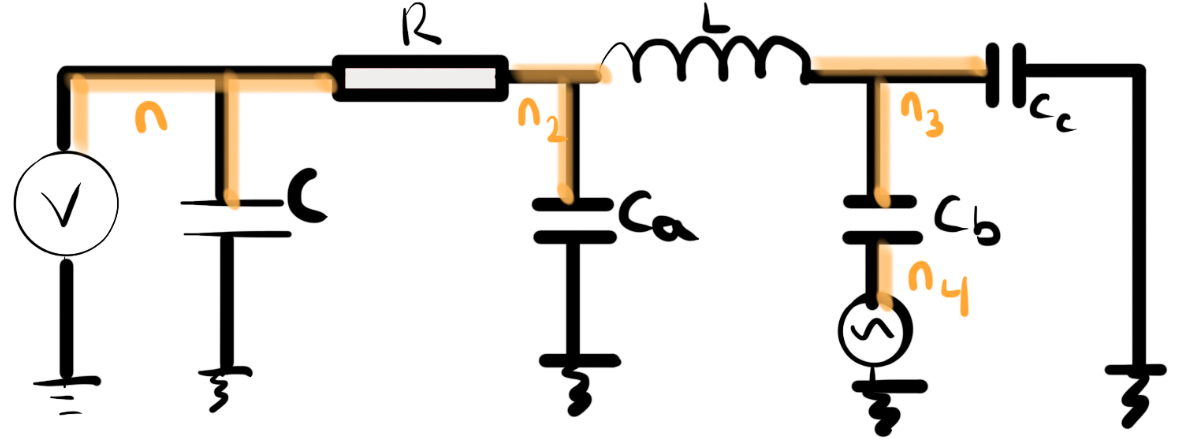
\includegraphics[height=5cm]{circuit_inverse_shapiro}
\end{figure}

\noindent

\noindent Constraints in this system are that we solve the current for
\begin{itemize}
\item Work with $ n $ \hfill number of CP of charge $ \mathbf{2e} $;
\item $ V $ \hfill the DC voltage that we fix;
\item $f$ \hfill is the frequency of the rf-bias.
\item \red{Ignore that large capacitance $ C $} - it's so large that it
  has no effect on the whole system.
\end{itemize}

\noindent Next  we write  out a system  of simultaneous  equations that
Oleg solves numerically in \verb|Mathematica| for $ n(t) $.

 \begin{equation}\label{key}
   \left\lbrace\begin{aligned}
       V & = \red{2eR\dot{n}} + \blue{\frac{2e}{C_a}n_2}\\
       V & = \red{L\frac{d}{dt}(\dot{n}-\dot{n}_2)} + \blue{\frac{2e}{C_b}(n_3 - n_4)}  \green{- V_{rf}\cos(2\pi ft)}\\
       V & = \red{L\frac{d}{dt}(\dot{n}-\dot{n}_2)} + \blue{\frac{2e}{C_c}n_3}
     \end{aligned}\right.
 \end{equation}
 \begin{itemize}
 \item  \red{Charge  passing  through  resistor $  R  $  and  inductor,
     $ V = L\dot{I} $};
 \item  \blue{Potential  difference  across  capacitors  due  to  onset
     charge};
 \item \green{RF-voltage source in action}.
 \end{itemize}

 \noindent  What  we  find  if   oscillations  in  this  charge  number
 $ n_1(t) $. Evaluating $ \iaverage{I(V)} = \int_{t_1}^{t_2}2e n(t)dt $
 for   different   bias    voltages   $   V   $,   we    can   plot   a
 $  V \text{  vs }  \iaverage{I(V)} $  graph, which  will show  Shapiro
 steps.

\begin{figure}[h]
  \centering 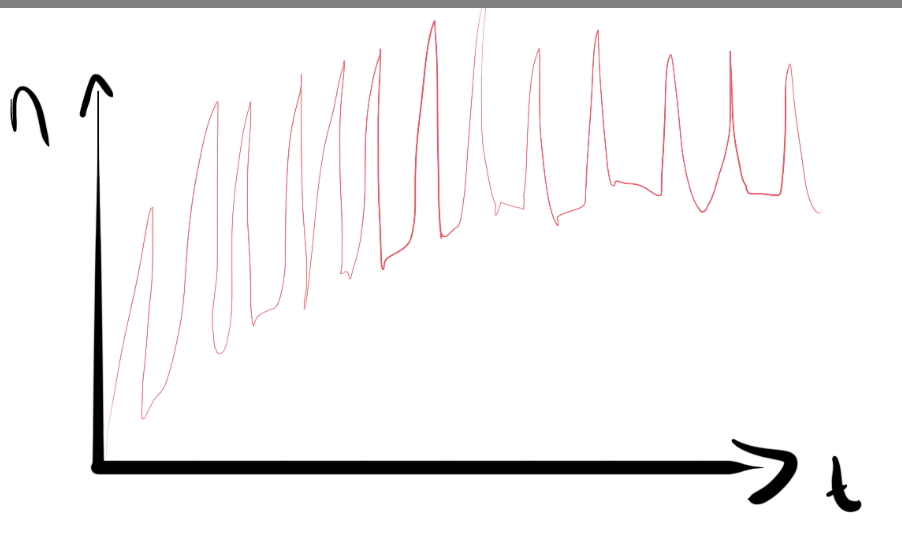
\includegraphics[height=4cm]{inverseShapiro_oscillations}
\end{figure}

\newpage
